\iffalse
\documentclass[journal,12pt,twocolumn]{IEEEtran}
\usepackage{setspace}
\usepackage{gensymb}
\singlespacing
\usepackage[cmex10]{amsmath}
\usepackage{amsthm}
\usepackage{mathrsfs}
\usepackage{txfonts}
\usepackage{stfloats}
\usepackage{bm}
\usepackage{cite}
\usepackage{cases}
\usepackage{subfig}
\usepackage{longtable}
\usepackage{multirow}
\usepackage{enumitem}
\usepackage{mathtools}
\usepackage{tikz}
\usepackage{circuitikz}
\usepackage{verbatim}
\usepackage[breaklinks=true]{hyperref}
\usepackage{tkz-euclide} % loads  TikZ and tkz-base
\usepackage{listings}
\usepackage{color}    
\usepackage{array}    
\usepackage{longtable}
\usepackage{calc}     
\usepackage{multirow} 
\usepackage{hhline}   
\usepackage{ifthen}   
\usepackage{lscape}     
\usepackage{chngcntr}
\DeclareMathOperator*{\Res}{Res}
\renewcommand\thesection{\arabic{section}}
\renewcommand\thesubsection{\thesection.\arabic{subsection}}
\renewcommand\thesubsubsection{\thesubsection.\arabic{subsubsection}}

\renewcommand\thesectiondis{\arabic{section}}
\renewcommand\thesubsectiondis{\thesectiondis.\arabic{subsection}}
\renewcommand\thesubsubsectiondis{\thesubsectiondis.\arabic{subsubsection}}
\renewcommand\thetable{\arabic{table}}
% correct bad hyphenation here
\hyphenation{op-tical net-works semi-conduc-tor}
\def\inputGnumericTable{}                                 %%

\lstset{
%language=C,
frame=single, 
breaklines=true,
columns=fullflexible
}
%\lstset{
%language=tex,
%frame=single, 
%breaklines=true
%}

\begin{document}
\newtheorem{theorem}{Theorem}[section]
\newtheorem{problem}{Problem}
\newtheorem{proposition}{Proposition}[section]
\newtheorem{lemma}{Lemma}[section]
\newtheorem{corollary}[theorem]{Corollary}
\newtheorem{example}{Example}[section]
\newtheorem{definition}[problem]{Definition}
\newcommand{\BEQA}{\begin{eqnarray}}
\newcommand{\EEQA}{\end{eqnarray}}
\newcommand{\define}{\stackrel{\triangle}{=}}
\bibliographystyle{IEEEtran}
\providecommand{\mbf}{\mathbf}
\providecommand{\pr}[1]{\ensuremath{\Pr\left(#1\right)}}
\providecommand{\qfunc}[1]{\ensuremath{Q\left(#1\right)}}
\providecommand{\sbrak}[1]{\ensuremath{{}\left[#1\right]}}
\providecommand{\lsbrak}[1]{\ensuremath{{}\left[#1\right.}}
\providecommand{\rsbrak}[1]{\ensuremath{{}\left.#1\right]}}
\providecommand{\brak}[1]{\ensuremath{\left(#1\right)}}
\providecommand{\lbrak}[1]{\ensuremath{\left(#1\right.}}
\providecommand{\rbrak}[1]{\ensuremath{\left.#1\right)}}
\providecommand{\cbrak}[1]{\ensuremath{\left\{#1\right\}}}
\providecommand{\lcbrak}[1]{\ensuremath{\left\{#1\right.}}
\providecommand{\rcbrak}[1]{\ensuremath{\left.#1\right\}}}
\theoremstyle{remark}
\newtheorem{rem}{Remark}
\newcommand{\sgn}{\mathop{\mathrm{sgn}}}
\providecommand{\abs}[1]{\left\vert#1\right\vert}
\providecommand{\res}[1]{\Res\displaylimits_{#1}} 
\providecommand{\norm}[1]{\left\lVert#1\right\rVert}
\providecommand{\mtx}[1]{\mathbf{#1}}
\providecommand{\mean}[1]{E\left[ #1 \right]}
\providecommand{\fourier}{\overset{\mathcal{F}}{ \rightleftharpoons}}
\providecommand{\system}[1]{\overset{\mathcal{#1}}{ \longleftrightarrow}}
\newcommand{\solution}{\noindent \textbf{Solution: }}
\newcommand{\cosec}{\,\text{cosec}\,}
\providecommand{\dec}[2]{\ensuremath{\overset{#1}{\underset{#2}{\gtrless}}}}
\newcommand{\myvec}[1]{\ensuremath{\begin{pmatrix}#1\end{pmatrix}}}
\newcommand{\mydet}[1]{\ensuremath{\begin{vmatrix}#1\end{vmatrix}}}
\let\vec\mathbf
\def\putbox#1#2#3{\makebox[0in][l]{\makebox[#1][l]{}\raisebox{\baselineskip}[0in][0in]{\raisebox{#2}[0in][0in]{#3}}}}
     \def\rightbox#1{\makebox[0in][r]{#1}}
     \def\centbox#1{\makebox[0in]{#1}}
     \def\topbox#1{\raisebox{-\baselineskip}[0in][0in]{#1}}
     \def\midbox#1{\raisebox{-0.5\baselineskip}[0in][0in]{#1}}

\vspace{3cm}
\title{Optimization Assignment}
\author{Gautam Singh}
\maketitle
\bigskip

\begin{abstract}
    This document contains the solution to Question 4 of Exercise 2 in Chapter
    10 of the class 11 NCERT textbook.
\end{abstract}

\begin{enumerate}
   
    \solution 
    \fi
		Any point on \eqref{eq:11/10/3/14/conv/line} is clearly of the form
    \begin{align}
        \vec{Q} = \vec{A} + \lambda\vec{m}
        \label{eq:11/10/3/14/conv/Q-def}
    \end{align}
    where $\lambda \in \mathbb{R}$ and
    \begin{align}
        \vec{A} = \myvec{0\\-4},\ \vec{m} = \myvec{4\\3}
        \label{eq:11/10/3/14/conv/vals}
    \end{align}
    Thus,
    \begin{align}
        f\brak{\lambda} &= \norm{\vec{Q}-\vec{P}}^2 \\
                        &= \norm{\vec{A}-\vec{P}+\lambda\vec{m}}^2 \\
                        &= \norm{\vec{m}}^2\lambda^2 + 2\vec{m}^\top\brak{\vec{A}-\vec{P}}\lambda + \norm{\vec{A}-\vec{P}}^2
                        \label{eq:11/10/3/14/conv/dist-lambda}
    \end{align}
    Since the coefficient of $\lambda^2$ in $f(\lambda)$ is positive, it
    follows that $f\brak{\lambda}$ is convex. Hence, the minima is achieved at
    \begin{align}
        f'\brak{\lambda_m} &= 2\brak{\norm{\vec{m}}^2\lambda_m + \vec{m}^\top\brak{\vec{A}-\vec{P}}} = 0 \\
        \implies \lambda_m &= -\frac{\vec{m}^\top\brak{\vec{A}-\vec{P}}}{\norm{\vec{m}}^2}
        \label{eq:11/10/3/14/conv/lambda-min}
    \end{align}
    Thus,
    \begin{align}
        \vec{Q_m} &= \vec{A} + \lambda_m\vec{m} \\
                  &= \vec{A} - \frac{\vec{m}^\top\brak{\vec{A}-\vec{P}}}{\norm{\vec{m}}^2}\vec{m}
                  \label{eq:11/10/3/14/conv/Q-m-exp}
    \end{align}
    Thus, substituting \eqref{eq:11/10/3/14/conv/vals} into \eqref{eq:11/10/3/14/conv/Q-m-exp}, we get
    \begin{align}
        \vec{Q_m} = \frac{1}{25}\myvec{68\\-49}
        \label{eq:11/10/3/14/conv/Q-sol}
    \end{align}
    The value of $\lambda_m$ is verified in Fig. \ref{fig:11/10/3/14/conv/convex}.
		\begin{figure}[!ht]
        \centering
        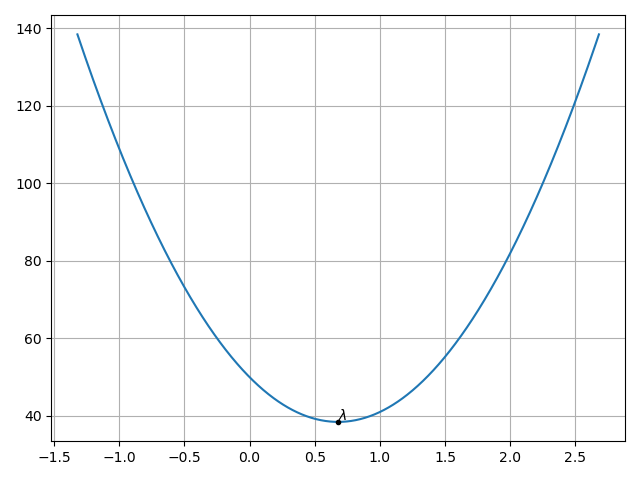
\includegraphics[width=\columnwidth]{11/10/3/14/conv/figs/convex.png}
        \caption{This convex function achieves its minimum at $\lambda_m$.}
        \label{fig:11/10/3/14/conv/convex}
    \end{figure}
